\section{Truth-level propagation and P1 results}\label{sec:p1}

The thickness law of Section~\ref{sec:string} was derived and checked on small controlled samples. This section tests it
on the full Stage-2 kinematics with $2.2\times10^5$ propagated events and compares the B-field thickness with the
multiple-scattering (MS) floor. Everything here is \textbf{truth level}: true hit positions, known hit-to-quirk assignment,
no pile-up, no resolution. Full detail is in \rep{sim/stage3/README.md} and \rep{sim/stage3/VALIDATION.md}; the numbers
are taken from \rep{sim/stage3/results/P1.json}.

\subsection{Propagation}\label{sec:p1:prop}
The Stage-3 kernel is the causal piecewise-null NG propagator of Section~\ref{sec:string:numerics} extended with
material effects: Bethe ionisation loss with straggling, Highland multiple scattering~\cite{Highland:1975pq} and the
magnetic kick, applied to each end; it reproduces the Stage-1 kernel bit for bit with material switched off. Hits are
recorded on 93 surfaces of a public CMS Phase-2 tracker layout (the tkLayout D111 configuration underlying
Ref.~\cite{CMS:2017lum}): the barrel and endcap Inner Tracker (IT), the stacked PS and 2S modules of the Outer Tracker
(OT), the barrel timing layer and ten virtual barrel layers for the P1 observable. The material is a per-layer slab of
1.2\% $X_0$ (IT barrel), 2.5\% (PS), 1.8\% (2S), 0.23\% for the beryllium beam pipe and 1.0\% for the IT service
cylinder (\UNV{}; varied by $\times0.5$ and $\times2$). The step parameter is $10^{-3}$ for field-only runs (at $10^{-2}$, $\DsB$ would be biased
by $+0.1$ to $+1.6\%$) and $10^{-2}$ with material. At $10^{-2}$ the out-of-plane hit displacement (median of the
per-event maximum) is 0.2--4$\um$ at $0.3$--$1\keV$ and $\le0.3\um$ at $2$--$3\keV$; the step-convergence test V3 (30
of 32 cells pass) covered field-only configurations. The material runs at $0.45$--$1.5\keV$ were not tested separately:
their field part carries up to $+1.6\%$ step bias, small against the multiple-scattering floor and the 3--20\% dip of
Section~\ref{sec:p1:ms}, and in the direction of quadrature, i.e.\ conservative for the dip (\EST{}).

The production comprised 4576 jobs and $218\,571$ events ($1.27\times10^7$ hits), split between two machines whose
kernel output is bit-identical in 224 of 225 overlap events (the exception differs by $4.4\um$). The P1 grid uses the
fermion at $\mQ=200,500,1000,1500\GeV$ and the scalar at $500\GeV$, $\Lam=0.45$--$10\keV$, $|\eta_{\rm pair}|<1$, the
vertex at the origin and 300 events per point (200 at 7 and $10\keV$). The same events are propagated in several
configurations: field only at $B_0$ and $B_0/2$ (giving $\DsB$ and, per event, $c=[\mathcal R(1/2)-1]/\ln2$), material only
($\DsMS$), field and material ($\DsBM$), the vacuum (a $\Ds\equiv0$ check) and the material variations.

\subsection{B-field thickness against the law}\label{sec:p1:law}
Figure~\ref{fig:p1law} and Table~\ref{tab:p1} compare the measured $\DsB$ and $c$ with the rotating-yo-yo model
evaluated on the same events. The primary statistic is the paired per-event ratio of measured to model thickness.
\begin{itemize}
\item \textbf{Thickness.} The paired median ratio is 0.990--1.002 for the fermion at $\mQ\ge500\GeV$ and
  $0.6$--$5\keV$, 0.966--0.990 at $200\GeV$ and 0.947--0.986 for the scalar: the model agrees per event to $\le3.4\%$
  (fermion) and $\le5.3\%$ (scalar), inside its declared 1--4\% accuracy for the fermion. The deviation is driven by
  $\gst$, not by spin: the ratio is within 0.8\% of one for $\gst<1.3$, 0.96--0.98 at $\gst=1.3$--1.6 and 0.89--0.93
  above. $\DsB$ is flat in $\mQ$ ($d\ln\DsB/d\ln\mQ=-0.004\ldots-0.07$ for $0.45$--$5\keV$).
\item \textbf{The $c$ law.} Per event, the law holds: in the pre-registered gate sample the paired agreement is
  $\le1\%$ at $1\keV$, and in the full production the conditional median of $c$ agrees with the event's prediction
  within $\pm1.5\%$ at $1$--$2\keV$ (every $\kB$ bin within $\pm2.4\%$). \textbf{The population median does not pass
  the pre-set gate}: at $1\keV$ it lies $+0.7/+2.0/+1.1/+2.1/+3.2\%$ above the prediction for $E$ 200/500/1000/1500 and
  $\Etil$ 500 (2.2--2.4$\sigma$ at the three failing points), against a pre-declared limit of $1.5\%$ at all five points
  (gate V2b, \rep{sim/stage3/VALIDATION.md}); pooled over $1$--$2\keV$ the excess is $+1.71\pm0.29\%$, and the same
  number appears in $\mathcal R(1/2)=1.0737\pm0.0007$ at $500\GeV$ (2.4$\sigma$ above 1.072). A zero-median symmetric
  per-event scatter reproduces it ($+2.04\%$), so we read it as an estimator effect (\EST{}); it is not a step effect.
  The user decided to proceed past the gate and to record it as a finding (\rep{LOG.md}, 2026-10-11). In dimensionless terms the law holds for median
  $\lmax/\RIT\lesssim0.6$ and $\kB\lesssim4$, with $\RIT\approx14.6\cm$ the outer IT barrel radius. At $0.45\keV$ it fails
  ($\kB$-ordered residuals from $+6\%$ to $-26\%$), where the non-secular $\Lam^{-4}$ terms omitted in the model matter
  and the pair does not turn around inside the IT. The $\Lam$ exponent $-2+2c$ is the asymptotic one ($\lmax\ll\RIT$). The measured slopes are steeper by
  3.9--5.9$\sigma$ for $0.6\to1\keV$ at all five points, by 4.1/4.5$\sigma$ for $1\to2\keV$ at $E$ 1500/$\Etil$ 500 and by
  3.0/3.4/3.9$\sigma$ for $1\to3\keV$ at $E$ 1000/$E$ 1500/$\Etil$ 500, i.e.\ wherever $\lmax/\RIT$ at the lower end
  reaches $\approx0.5$--0.6 (Table~\ref{tab:p1}); the edge of the validity window is therefore soft. The full
  event-level model agrees in every interval ($|{\rm pull}|\le2.6$).
\item \textbf{The $3$--$5\keV$ excess.} At $3$--$5\keV$ events with large $\kB$ carry a positive excess of $c$ whose size is
  measured: up to $+57\pm11\%$ at $5\keV$ for $\kB\ge10$ and $+3$ to $+5\%$ already at $\kB<4$; the population-median
  excess is $+6.2\pm0.5\%$. Its \textbf{attribution to the CM magnetic field is an estimate}: it grows with $\Nosc$ at matched
  $\kB$ and $\epsp$, and switching $\Bstar$ off in a dedicated run (160 events at $500$ and $1000\GeV$) removes the bulk
  of the population-median excess ($+1.8\pm0.7\%$ against $+9.7\pm1.3\%$ for the same masses, $5.5\sigma$; paired on the
  same events the difference is $+8.6\pm4.2\%$). With $\Bstar$ off, the residual is $\le3\%$ for $\kB<10$ and $+12\pm3\%$
  at $\kB\ge10$, inside the allowance for the double-precision floor of Section~\ref{sec:string:valid}. \textbf{The floor
  test (O-1) that would separate the two was not done.}
\item \textbf{Above $5\keV$.} The paired ratio rises to $1.016\pm0.005$ ($500\GeV$) and $1.027\pm0.005$ ($1000\GeV$) at
  $10\keV$, not carried by floor-flagged events; this turns part of the unattributed $\pm5\%$ of
  Section~\ref{sec:string:valid} into a measured $+1.6\%/+2.7\%$, of the same sign as the $c$ excess.
\end{itemize}

\begin{figure}[htbp]
\centering
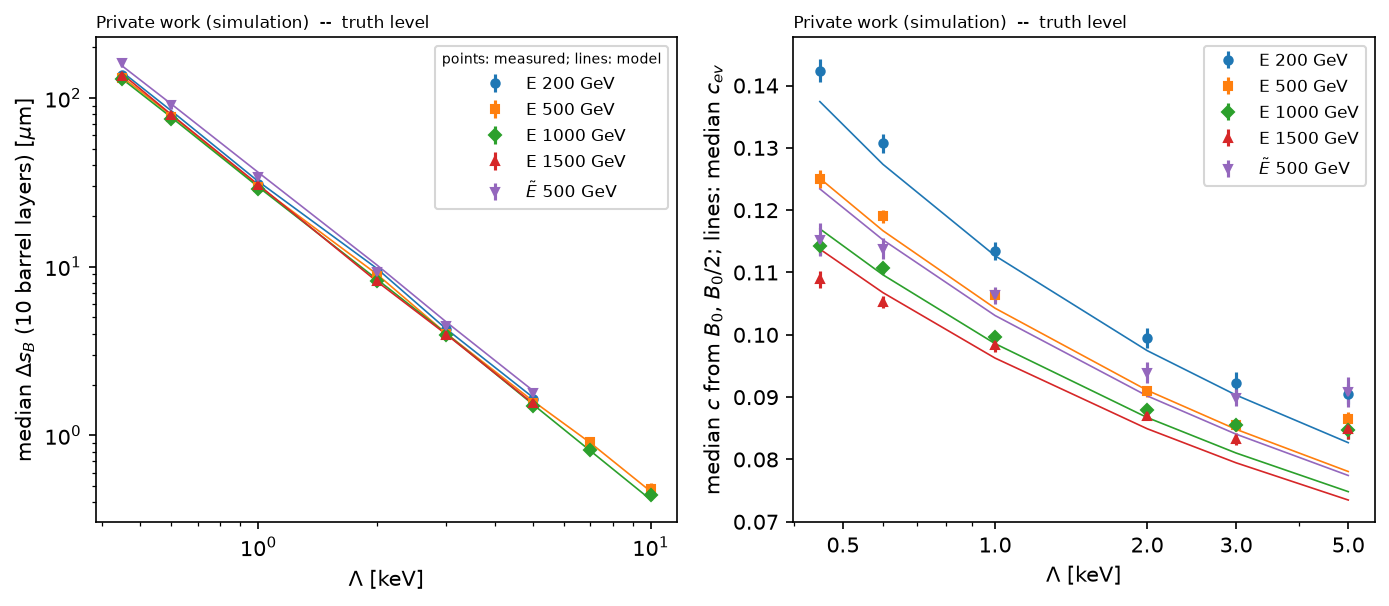
\includegraphics[width=0.98\linewidth,height=0.40\linewidth]{figures/S3_p1_dsB_c.png}
\caption{P1 at truth level (field only, no material, $|\eta_{\rm pair}|<1$, vertex at the origin, ten barrel layers;
Stage-3 diagnostic figure). (Left) Median B-field plane thickness $\DsB$ against $\Lam$ for the five (species, mass) points:
points are the propagation, lines the rotating-yo-yo model on the same events; the curves fall as $\approx\Lam^{-1.8}$
and are nearly independent of $\mQ$. (Right) Median local slope $c$ from paired $B_0$ and $B_0/2$ runs (points) and the
median per-event prediction $1/[\ln(1/\epsB)+C_{\rm ev}]$ (lines). The prediction is followed at $1$--$3\keV$; the
excess at $5\keV$ is the $\kB$-dependent effect discussed in the text, and the $0.45$--$0.6\keV$ deviations mark the
breakdown of the law where $\lmax$ approaches the IT radius.}
\label{fig:p1law}
\end{figure}

\begin{table}[htbp]
\centering
\footnotesize
\setlength{\tabcolsep}{4pt}
\caption{P1 at truth level at $\Lam=1$ and $5\keV$ (the $3\keV$ rows are in the source table) (Stage 3, \rep{sim/stage3/README.md} results table). ``ratio'' is the
paired per-event median $\DsB^{\rm meas}/\DsB^{\rm model}$ with its bootstrap error; $c$ is measured from $B_0$ and
$B_0/2$ and compared with the median per-event prediction $c_{\rm ev}$; $\DsMS$ is the material-only thickness and the
last column the measured $\DsBM/\sqrt{\DsB^2+\DsMS^2}$. Errors on $\DsB$ and $\DsMS$ are bootstrap errors of the median.}
\label{tab:p1}
\begin{tabular}{llccccccc}
\toprule
point & $\Lam$ & $\lmax/\RIT$ & $\DsB$ [$\mu$m] & ratio & $c$ (meas.) & $c_{\rm ev}$ & $\DsMS$ [$\mu$m] & BM\\
\midrule
$E$ 200  & 1 & 0.19  & $31.1\pm1.8$   & $0.986\pm0.001$ & $0.1135\pm0.0014$ & 0.1127 & $9.9\pm0.6$ & $0.97$\\
         & 5 & 0.0075& $1.64\pm0.09$  & $0.990\pm0.002$ & $0.0905\pm0.0016$ & 0.0827 & $11.3\pm0.6$ & $0.89$\\
$E$ 500  & 1 & 0.37  & $29.5\pm1.6$   & $0.993\pm0.001$ & $0.1064\pm0.0009$ & 0.1043 & $13.2\pm1.1$ & $0.94$\\
         & 5 & 0.015 & $1.56\pm0.08$  & $0.997\pm0.001$ & $0.0865\pm0.0011$ & 0.0781 & $15.5\pm1.0$ & $0.99$\\
$E$ 1000 & 1 & 0.52  & $28.7\pm1.5$   & $0.998\pm0.001$ & $0.0996\pm0.0008$ & 0.0986 & $18.2\pm1.2$ & $0.95$\\
         & 5 & 0.021 & $1.49\pm0.08$  & $1.000\pm0.001$ & $0.0848\pm0.0015$ & 0.0748 & $22.3\pm1.5$ & $0.93$\\
$E$ 1500 & 1 & 0.61  & $30.4\pm1.1$   & $0.999\pm0.001$ & $0.0983\pm0.0010$ & 0.0963 & $22.8\pm1.5$ & $0.93$\\
         & 5 & 0.024 & $1.56\pm0.05$  & $1.002\pm0.000$ & $0.0848\pm0.0016$ & 0.0735 & $24.5\pm2.0$ & $1.09$\\
$\Etil$ 500 & 1 & 0.59 & $33.9\pm2.3$ & $0.969\pm0.005$ & $0.1063\pm0.0014$ & 0.1031 & $14.5\pm1.3$ & $0.95$\\
         & 5 & 0.024 & $1.79\pm0.12$  & $0.952\pm0.008$ & $0.0908\pm0.0024$ & 0.0774 & $14.3\pm0.9$ & $1.03$\\
\bottomrule
\end{tabular}
\end{table}

\subsection{The multiple-scattering floor and the combination of B and MS}\label{sec:p1:ms}
With material, the plane thickness has a floor that is nearly independent of $\Lam$: the median $\DsMS$ is $\approx10$,
13--16, 17--22, 18--28 and 12--16$\um$ for $E$ at $200/500/1000/1500\GeV$ and $\Etil$ at $500\GeV$ (truth level,
nominal material). It rises with $\mQ$ because heavier pairs are slower and scatter more. The material scaling exponents
$\ln[\DsMS(\times2)/\DsMS(\times0.5)]/\ln4$ are 0.36--0.62, against $\approx0.5$ expected from the Highland $\sqrt{x/X_0}$
scaling~\cite{Highland:1975pq,ParticleDataGroup:2024cfk} ($\chi^2=26.0/10$ against the single-point code-scaling value
0.517; the $1000$ and $1500\GeV$ points are low by 2--2.6$\sigma$). The crossover $\DsB=\DsMS$ falls with mass:
$\Lcross=1.91/1.50/1.25/1.16\keV$ for $E$ at $200/500/1000/1500\GeV$ and $1.59\keV$ for $\Etil$. Above $\Lcross$ the
coplanarity of a truth-level quirk pattern is limited by material, not by the field.

Figures~\ref{fig:u2} and~\ref{fig:u2ratio} show how the two effects combine. Per event they add
\emph{below quadrature} in the crossover region: the median of $\DsBM/\sqrt{\DsB^2+\DsMS^2}$ is 0.99--1.00 at $0.45\keV$,
0.95--1.00 at $0.6\keV$ and 0.80--0.97 at $1$--$3\keV$ (lowest: $E$ 200 at $3\keV$, $0.804\pm0.042$), and consistent with
one within $2\sigma$ at $5$--$10\keV$; the dip is deepest at $\Lam/\Lcross=1.25$--1.73. The ratio to the linear sum is
0.62--1.00. No combination rule is fitted; the measured ratios are reported as they are (user decision, Appendix~\ref{app:limits}).

\begin{figure}[htbp]
\centering
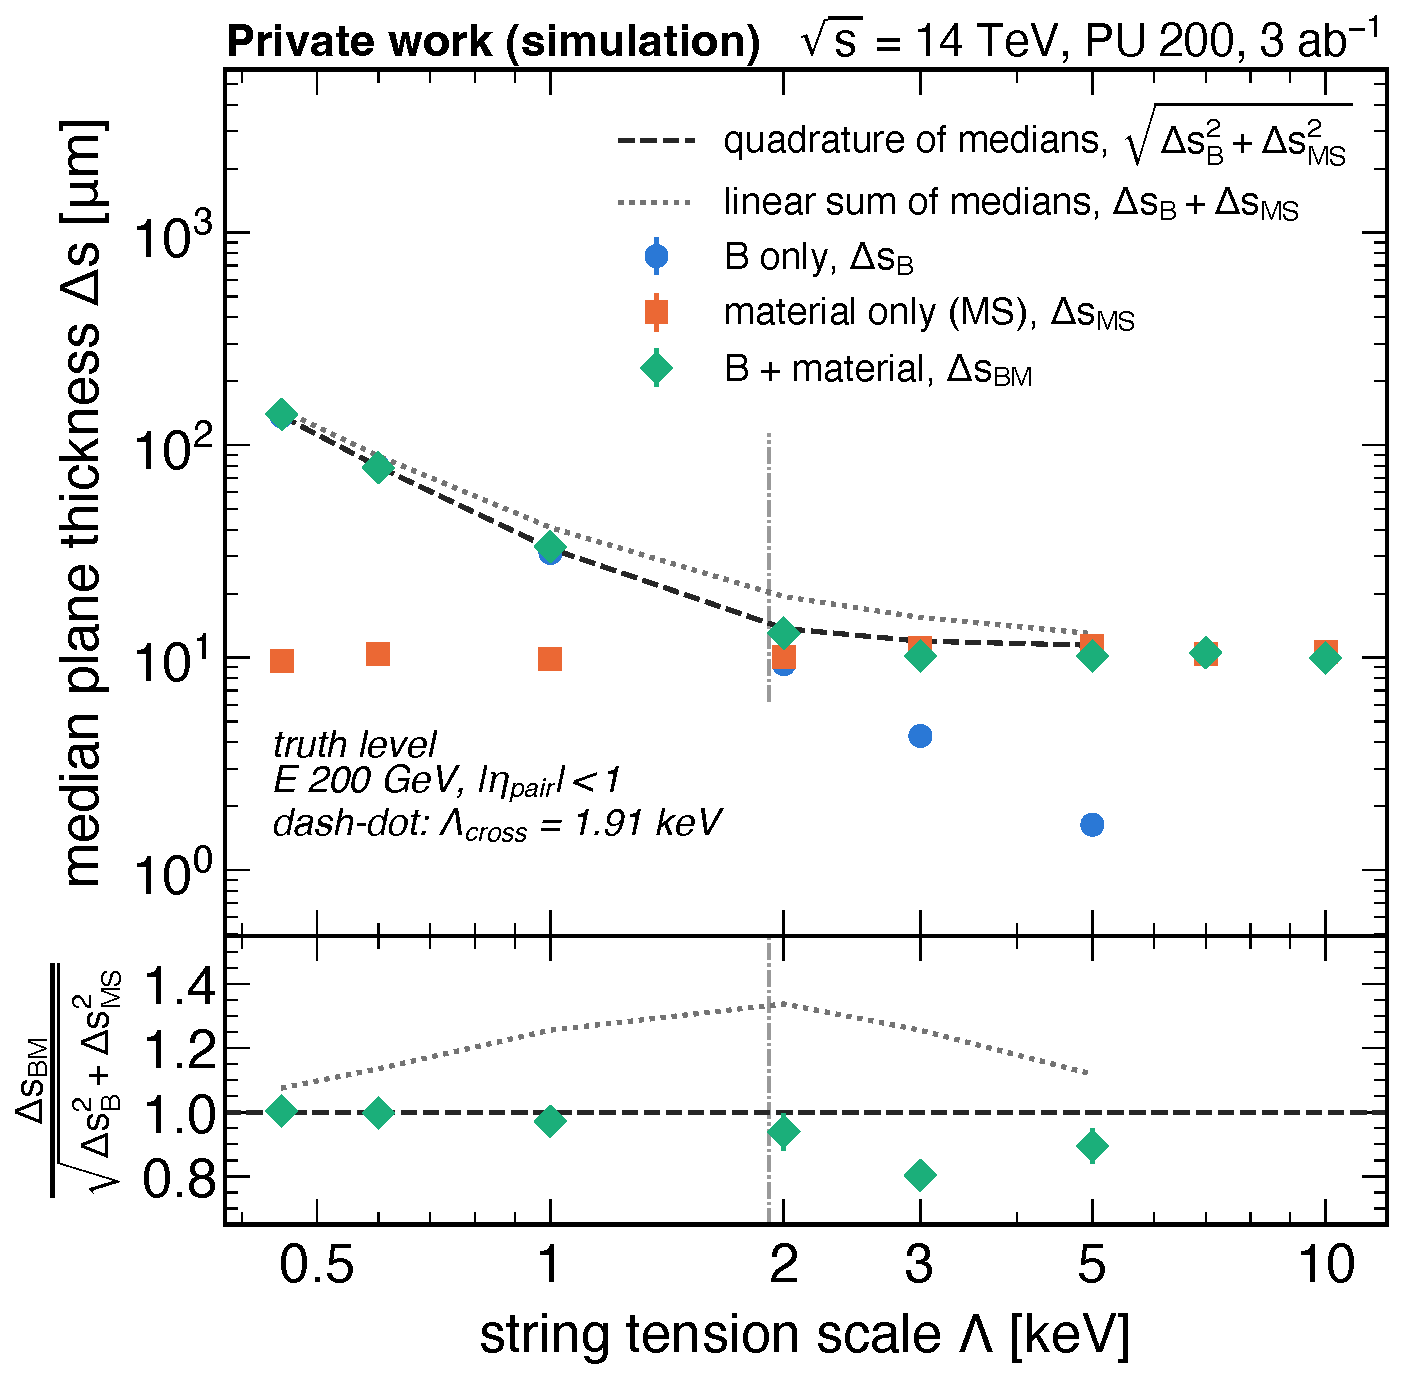
\includegraphics[height=0.34\linewidth]{figures/T1_u2_thickness_F_m200.pdf}\hspace{0.02\linewidth}
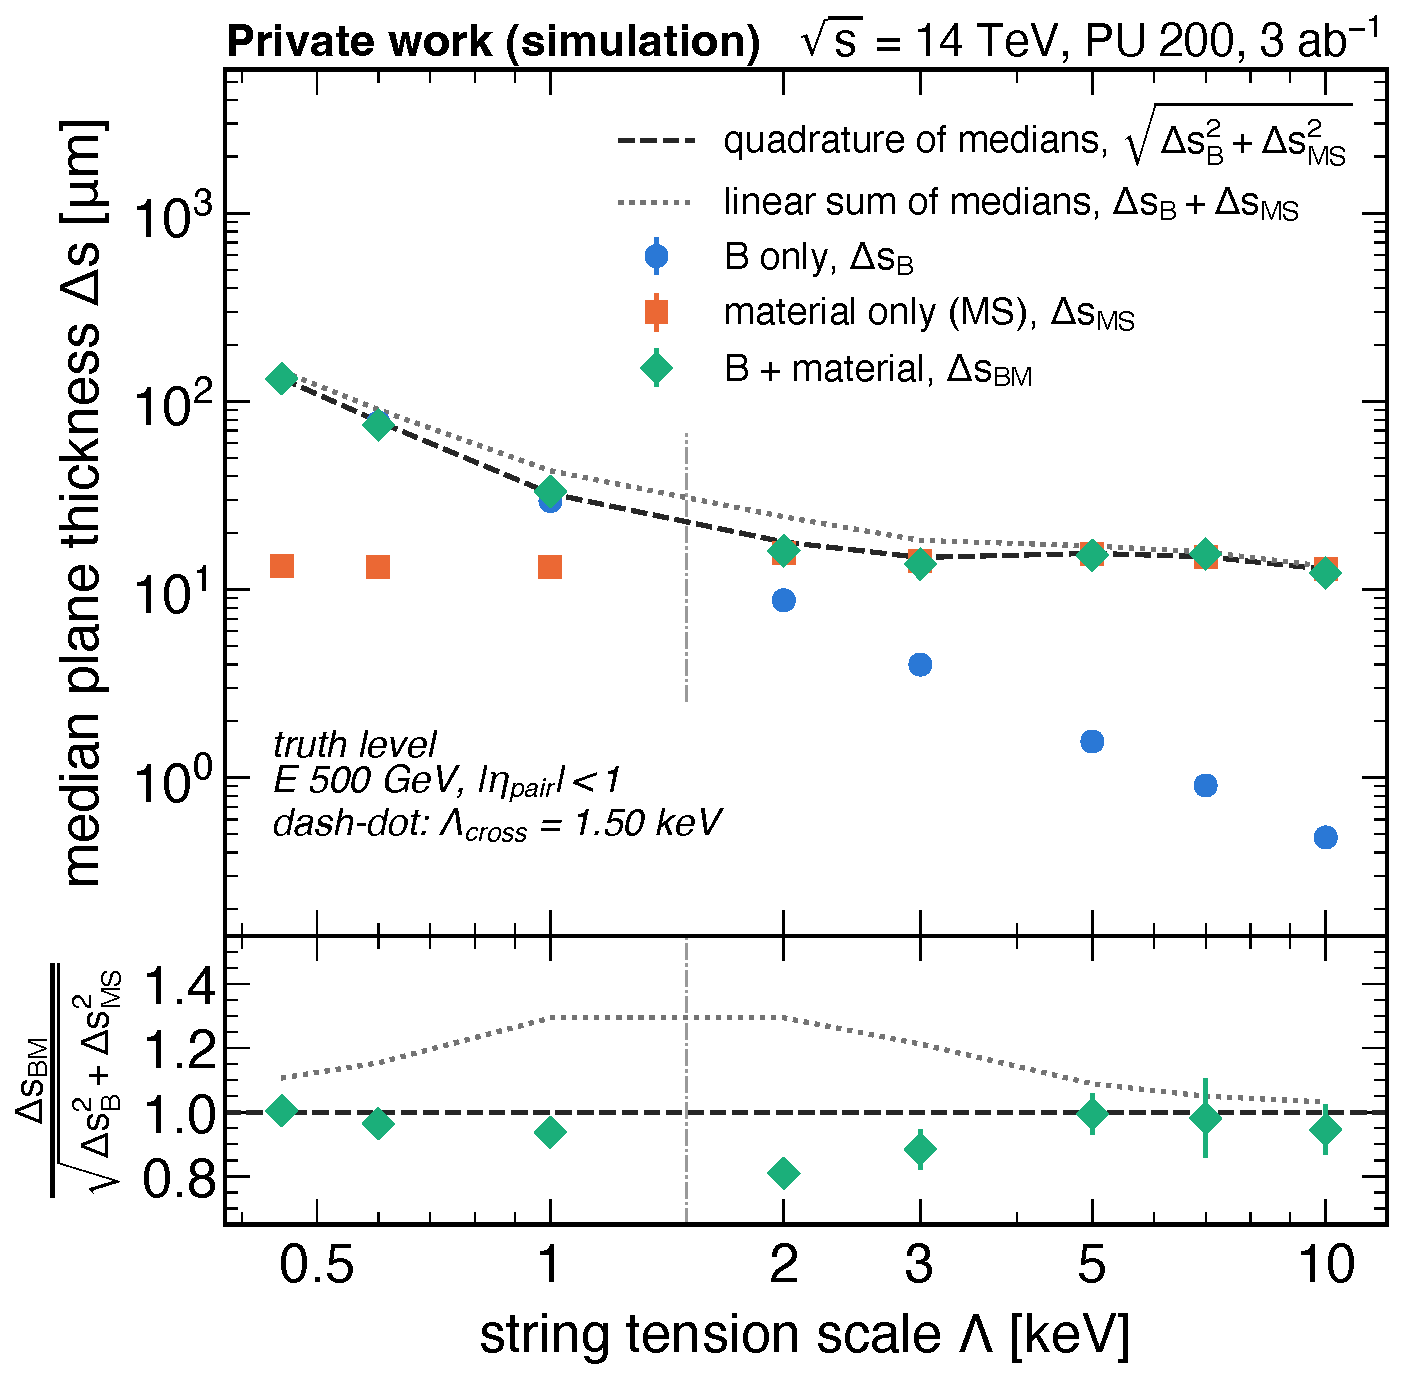
\includegraphics[height=0.34\linewidth]{figures/T1_u2_thickness_F_m500.pdf}\\[4pt]
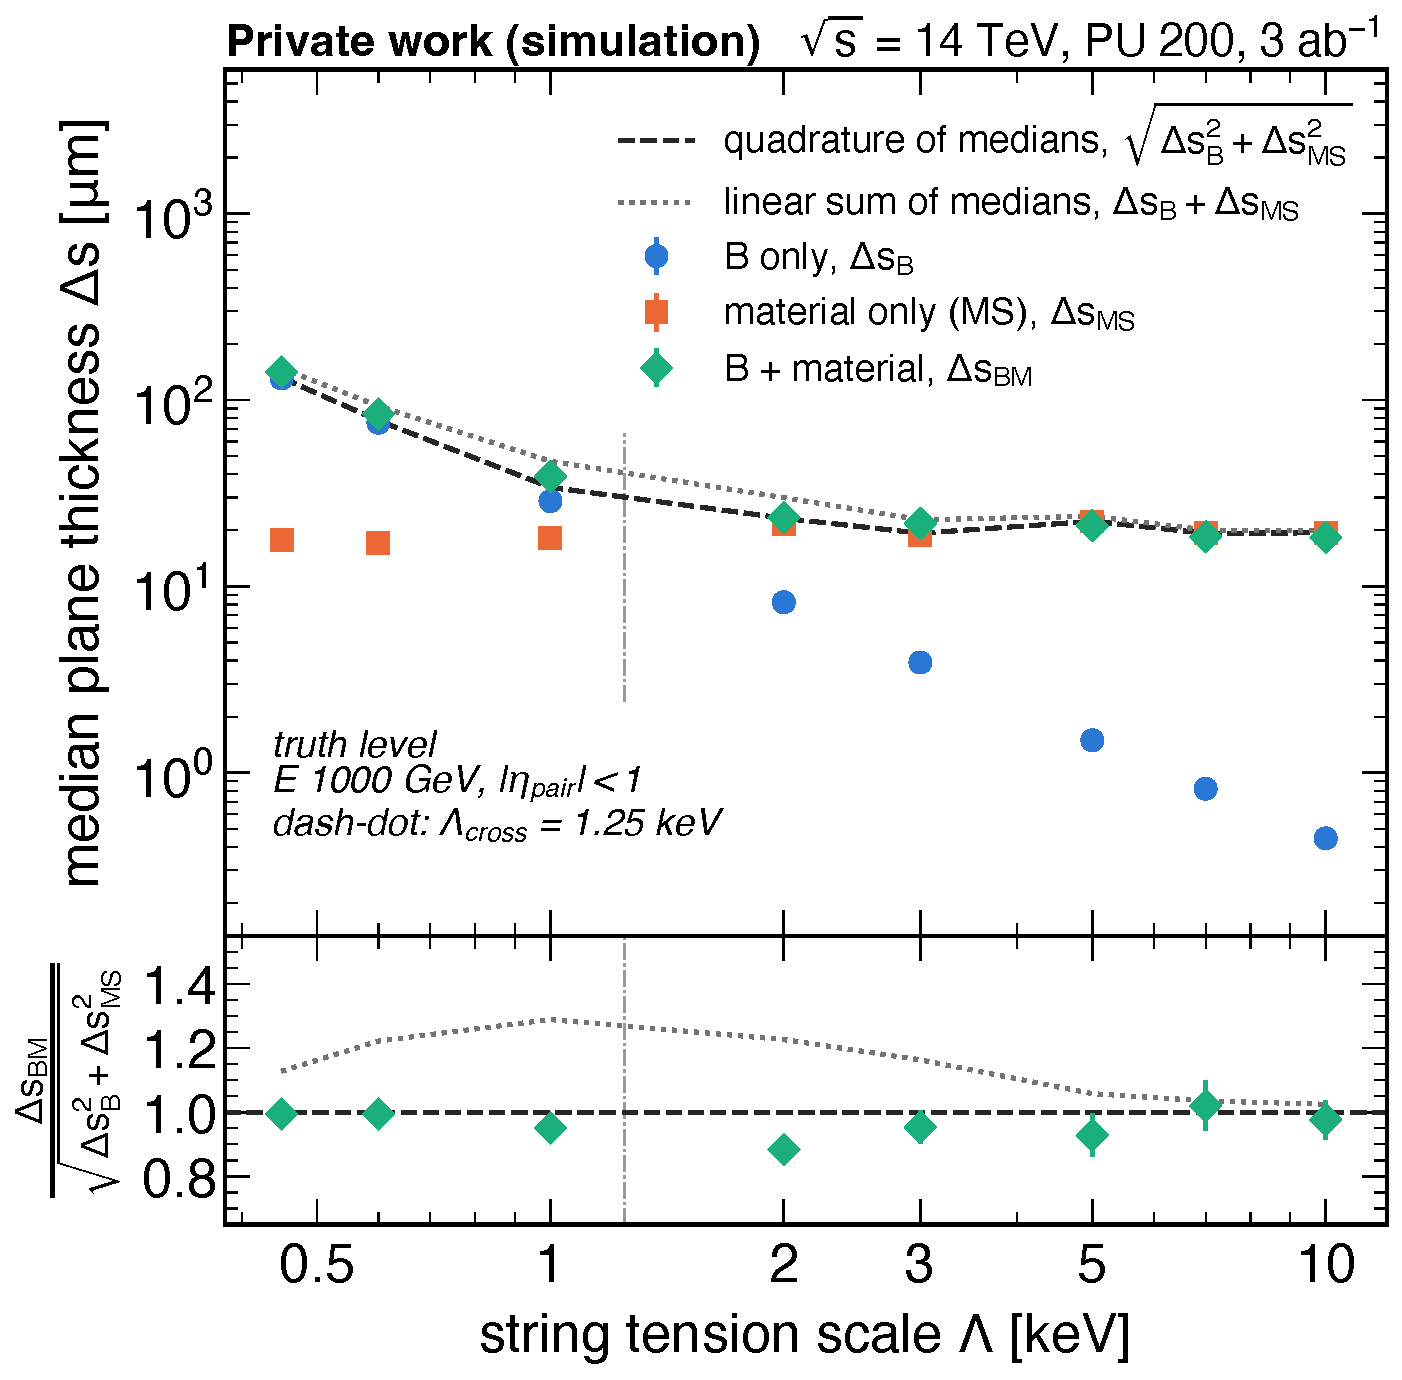
\includegraphics[height=0.34\linewidth]{figures/T1_u2_thickness_F_m1000.pdf}\hspace{0.02\linewidth}
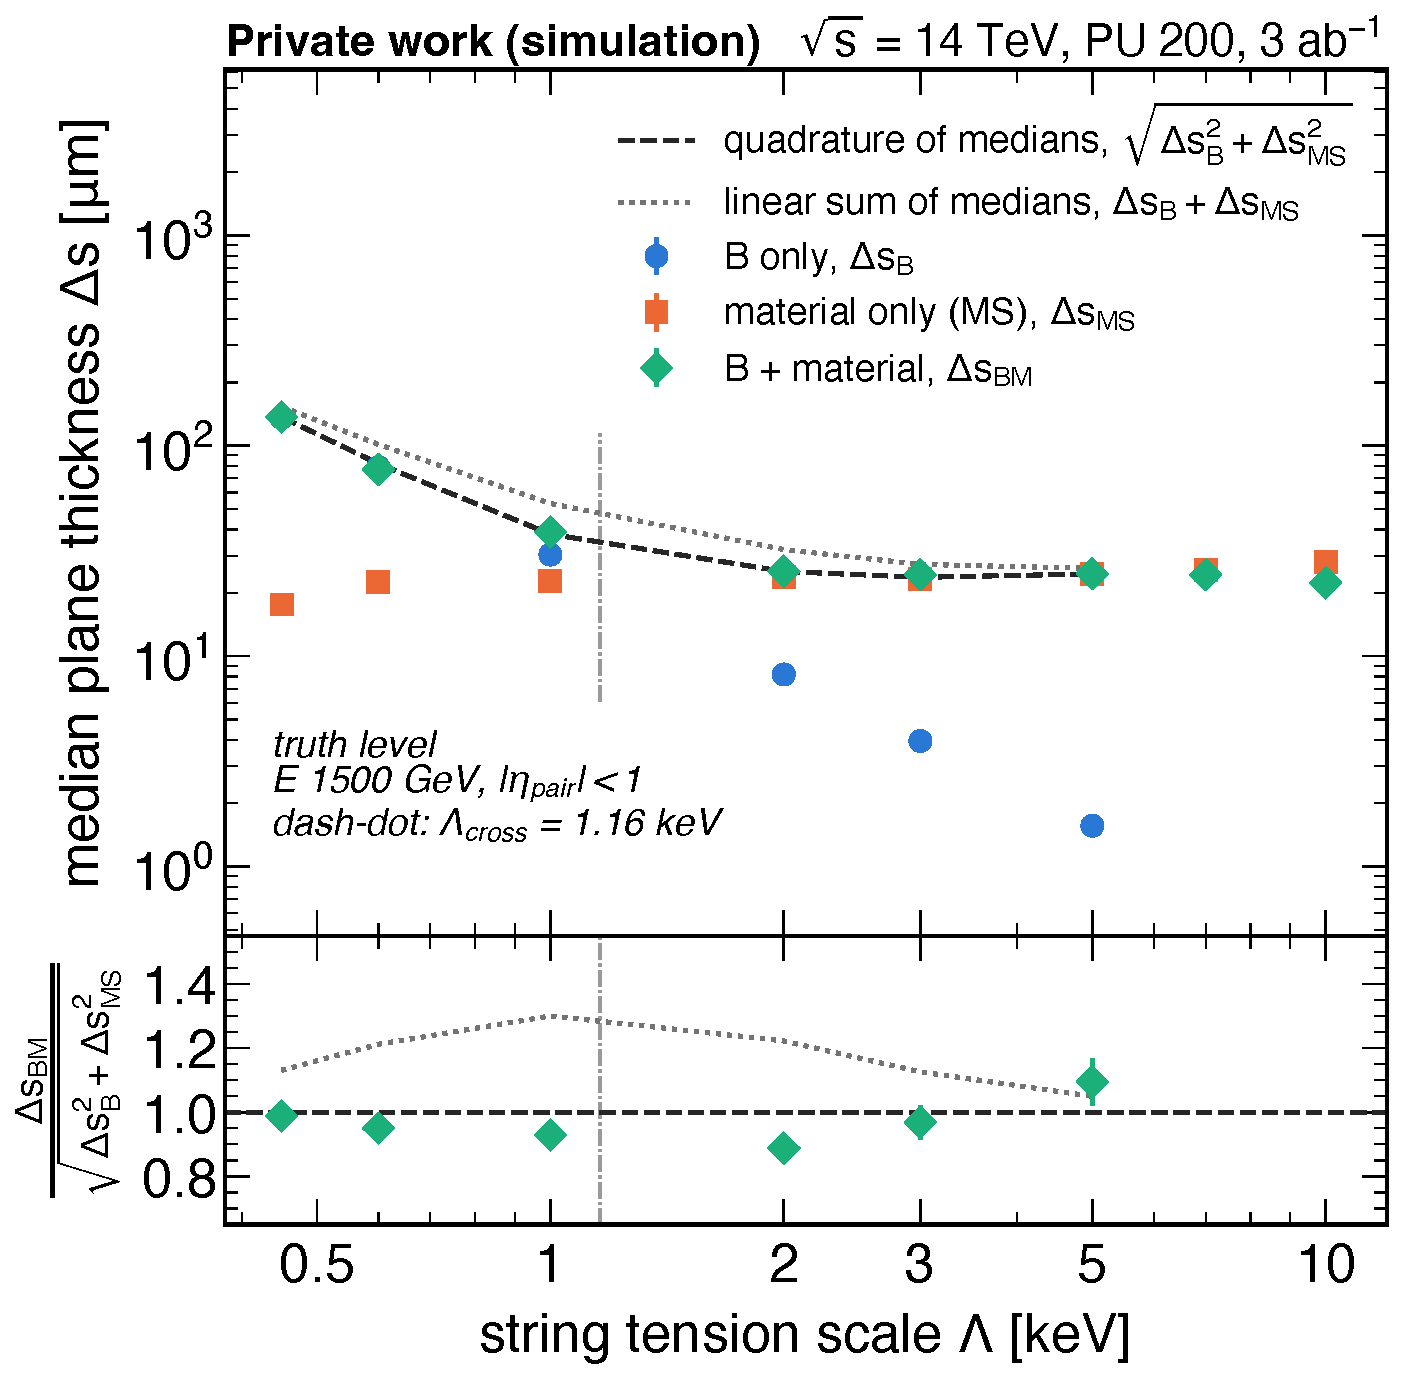
\includegraphics[height=0.34\linewidth]{figures/T1_u2_thickness_F_m1500.pdf}
\caption{B-field and multiple-scattering plane thickness at truth level for the fermion at $\mQ=200$ (top left), 500
(top right), 1000 (bottom left) and $1500\GeV$ (bottom right), $|\eta_{\rm pair}|<1$. Upper panels: median $\DsB$
(field only), $\DsMS$ (material only) and $\DsBM$ (both) against $\Lam$, with the quadrature and linear sums of the
medians; the dash-dot line marks $\Lcross$. Lower panels: $\DsBM$ over the quadrature sum. The field dominates below
$\Lcross\approx1.2$--$1.9\keV$ and the floor above; in the crossover region the two add below quadrature. Pile-up is
not simulated at truth level; the right-hand label gives the HL-LHC conditions of the study. The scalar ($\Etil$ at
$500\GeV$) behaves the same way (\rep{paper/figures/T1_u2_thickness_S_m500.pdf}).}
\label{fig:u2}
\end{figure}

\begin{figure}[htbp]
\centering
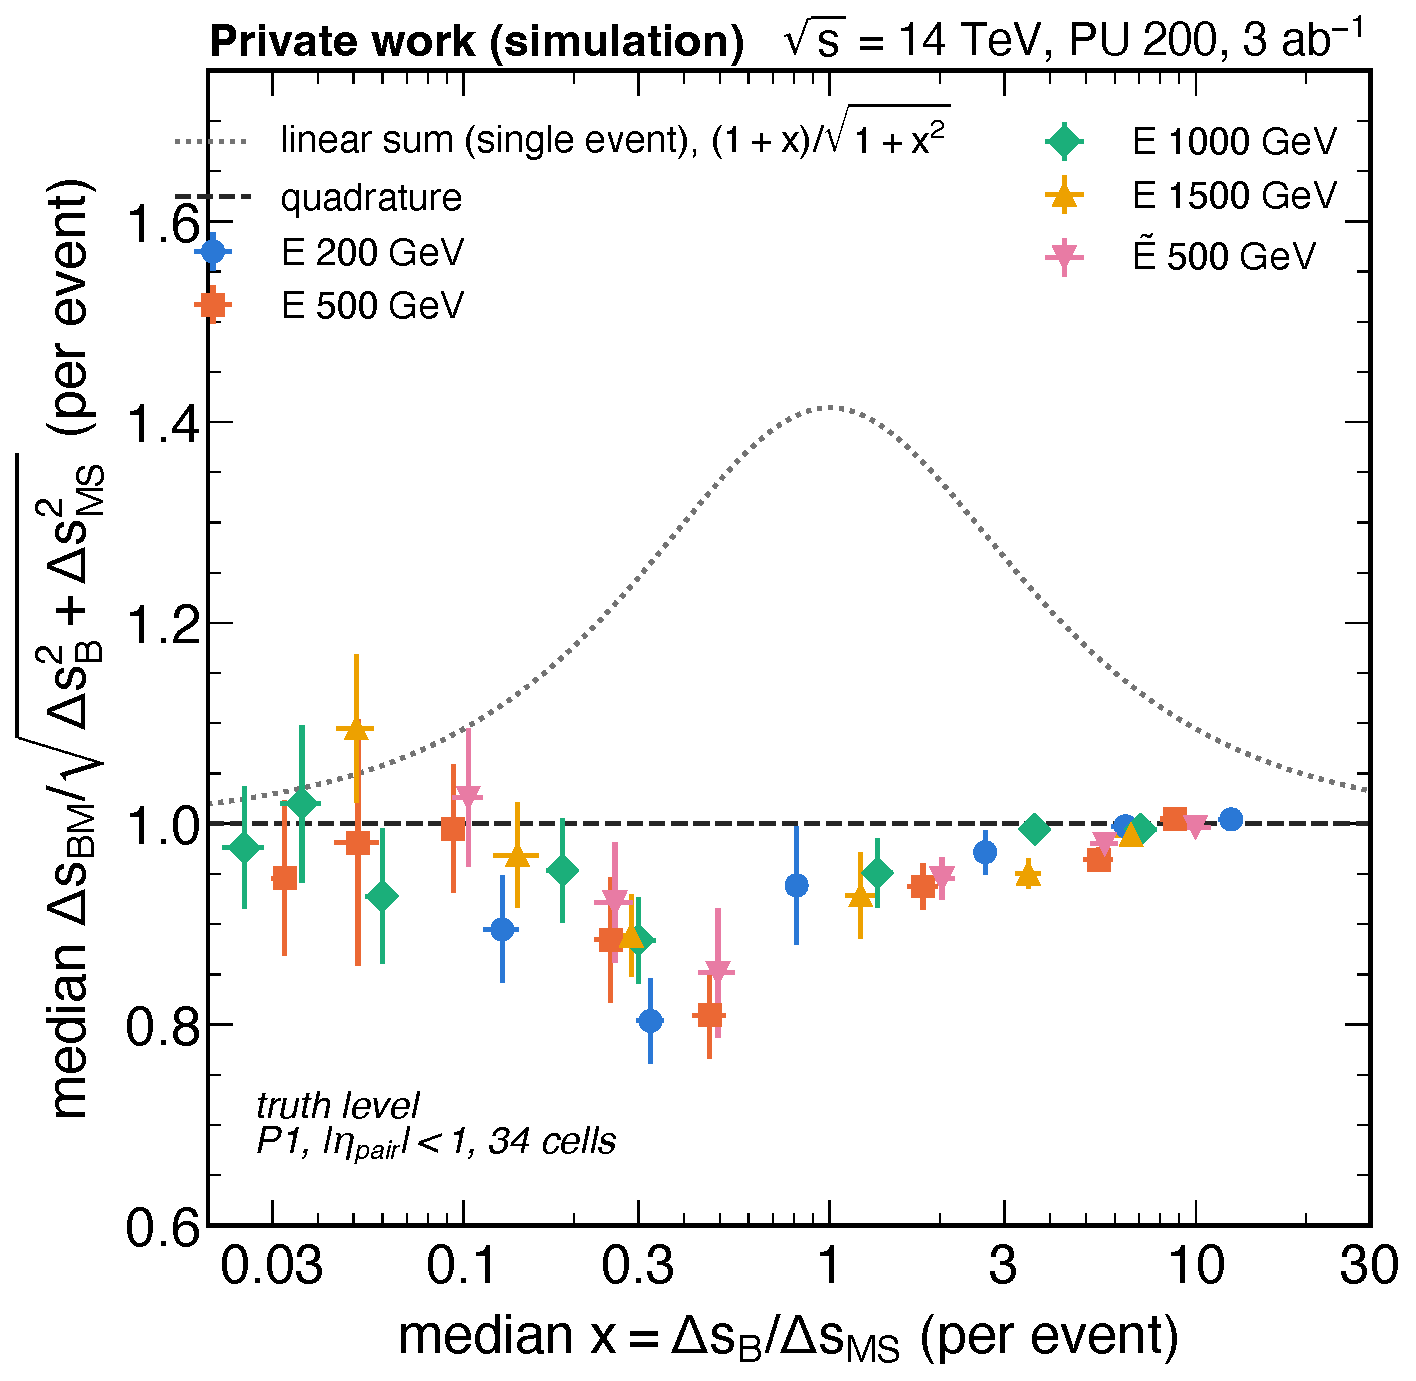
\includegraphics[height=0.37\linewidth]{figures/T2_u2_ratio_vs_x.pdf}\hspace{0.02\linewidth}
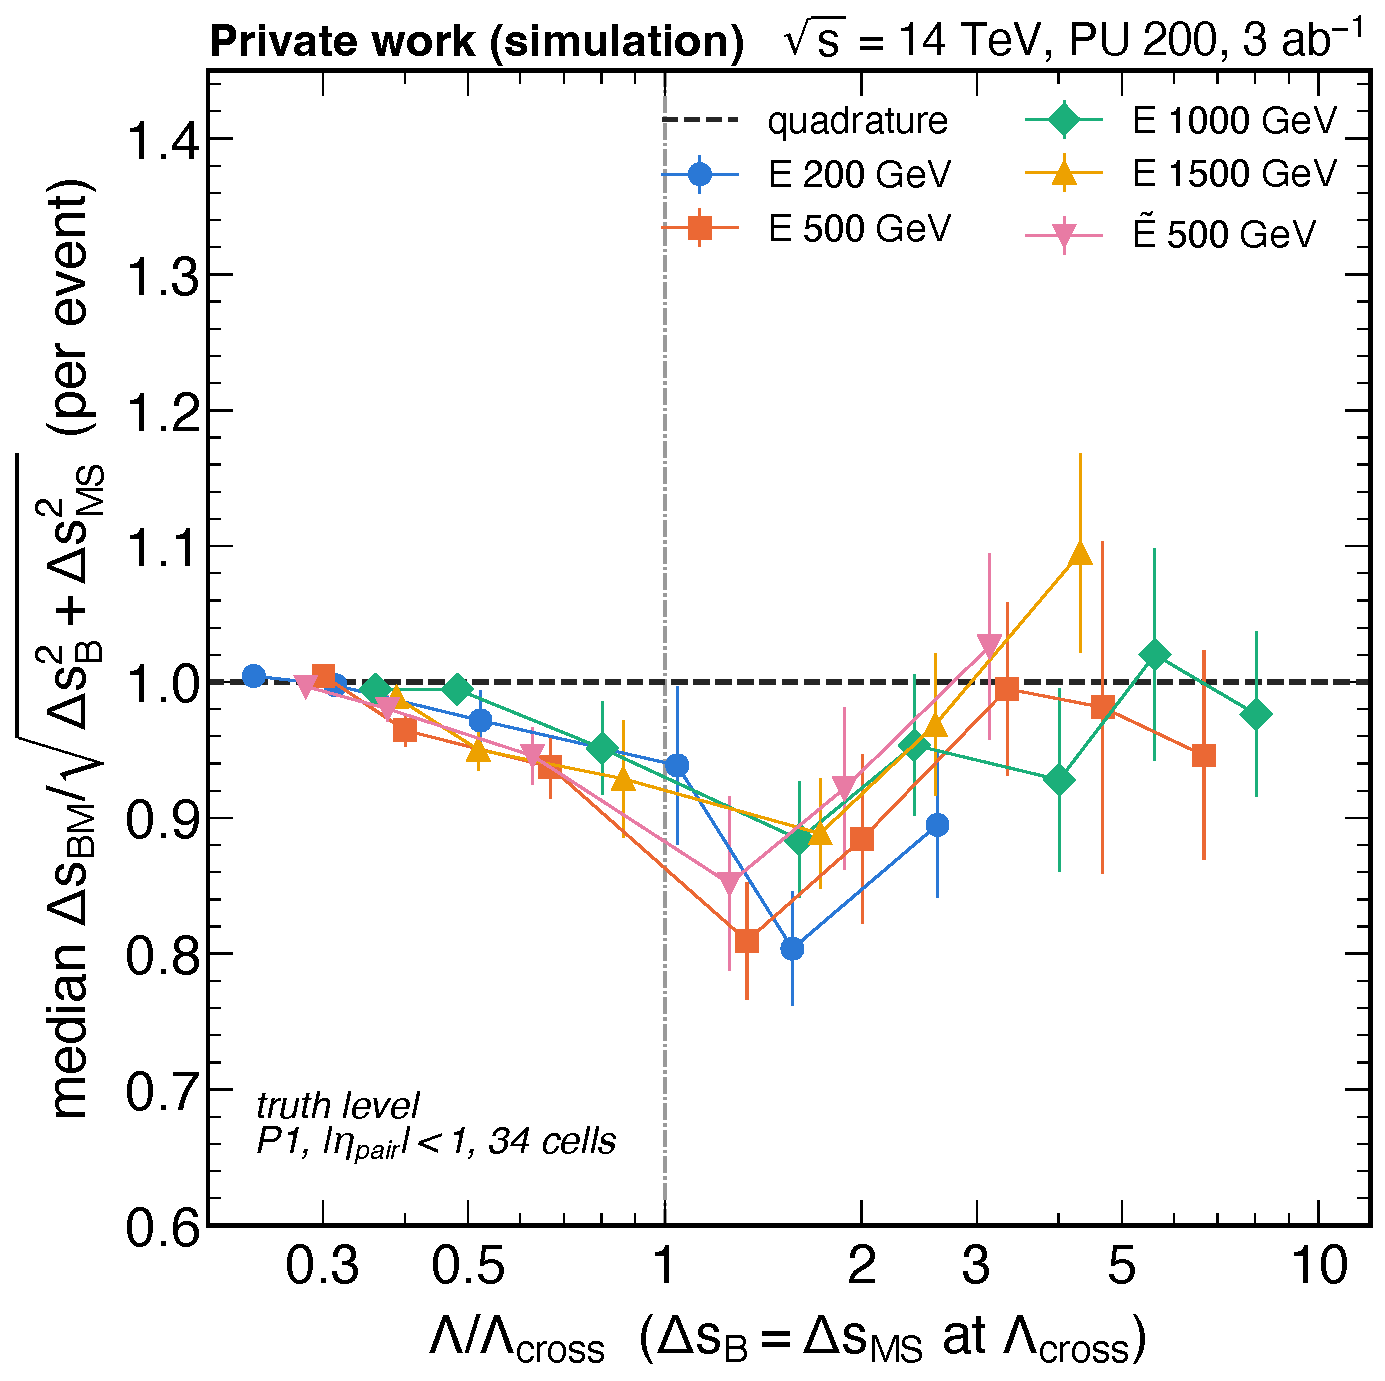
\includegraphics[height=0.37\linewidth]{figures/T3_u2_ratio_vs_lamcross.pdf}
\caption{Combination of the B-field and multiple-scattering thickness at truth level, all 34 cells of the P1 grid with
both measurements. (Left) Measured median $\DsBM/\sqrt{\DsB^2+\DsMS^2}$ against $x=\DsB/\DsMS$, with the curve for
a single event in which the two displacements add linearly. (Right) The same ratio against $\Lam/\Lcross$: the
sub-quadrature dip is deepest at $\Lam/\Lcross\approx1.25$--1.73. Pile-up is not simulated at truth level.}
\label{fig:u2ratio}
\end{figure}

\subsection{P1 in summary}\label{sec:p1:summary}
At truth level the B-field plane thickness of quirk pairs in the CMS solenoid is described by
$\DsB\propto\epsB[\ln(1/\epsB)+C]$, with a local slope $c\simeq0.10$--0.11 at $1\keV$ that falls with $\Lam$ as
predicted. The law is derived and confirmed by blind numerics at $1\keV$; on the full simulation it holds per event in
the window $\lmax/\RIT\lesssim0.6$, $\kB\lesssim4$, while the population median lies $+2$--$3\%$ above the prediction
at $1\keV$ (a failed $1.5\%$ gate, read as an estimator effect, \EST{}), and a larger $\kB$-dependent excess at
$3$--$5\keV$ is measured whose attribution to $\Bstar$ is estimated, not established. For $\Lam\gtrsim1.2$--$1.9\keV$
the thickness is set by multiple scattering at 10--28$\um$. Whether the B-field thickness survives at detector level was
not measured (user decision, Appendix~\ref{app:limits}): the detector-level study of Sections~\ref{sec:detector}--\ref{sec:mlam} uses the plane
thickness only through the finder tolerances.
